\documentclass[a4paper,twoside]{article}
\usepackage[T1]{fontenc}
\usepackage[bahasa]{babel}
\usepackage{graphicx}
\usepackage{graphics}
\usepackage{float}
\usepackage[cm]{fullpage}
\pagestyle{myheadings}
\usepackage{etoolbox}
\usepackage{setspace}
\usepackage{lipsum} 
\usepackage{indentfirst}
\setlength{\headsep}{30pt}
\usepackage[inner=2cm,outer=2.5cm,top=2.5cm,bottom=2cm]{geometry} %margin
% \pagestyle{empty}

\makeatletter
\renewcommand{\@maketitle} {\begin{center} {\LARGE \textbf{ \textsc{\@title}} \par} \bigskip {\large \textbf{\textsc{\@author}} }\end{center} }
\renewcommand{\thispagestyle}[1]{}
\markright{\textbf{\textsc{AIF401/AIF402 \textemdash Rencana Kerja Skripsi \textemdash Sem. Genap 2018/2019}}}

\onehalfspacing
 
\begin{document}

\title{\@judultopik}
\author{\nama \textendash \@npm} 

%tulis nama dan NPM anda di sini:
\newcommand{\nama}{Sandy Giovanni S.}
\newcommand{\@npm}{2015730041}
\newcommand{\@judultopik}{Integrasi \textit{Outlook Calendar} dan \textit{Slack}} % Judul/topik anda
\newcommand{\jumpemb}{1} % Jumlah pembimbing, 1 atau 2
\newcommand{\tanggal}{07/02/2019}

% Dokumen hasil template ini harus dicetak bolak-balik !!!!

\maketitle

\pagenumbering{arabic}

\section{Deskripsi}
Pada skripsi ini, akan dibuat sebuah perangkat lunak yang berfungsi untuk mengintegrasikan aplikasi \textit{Outlook Calendar} dan \textit{Slack}.\textit{ Outlook Calendar} sendiri adalah sebuah aplikasi buatan \textit{Microsoft} yang merupakan aplikasi manajemen kalender \textit{online}. 

\begin{figure}[h]
  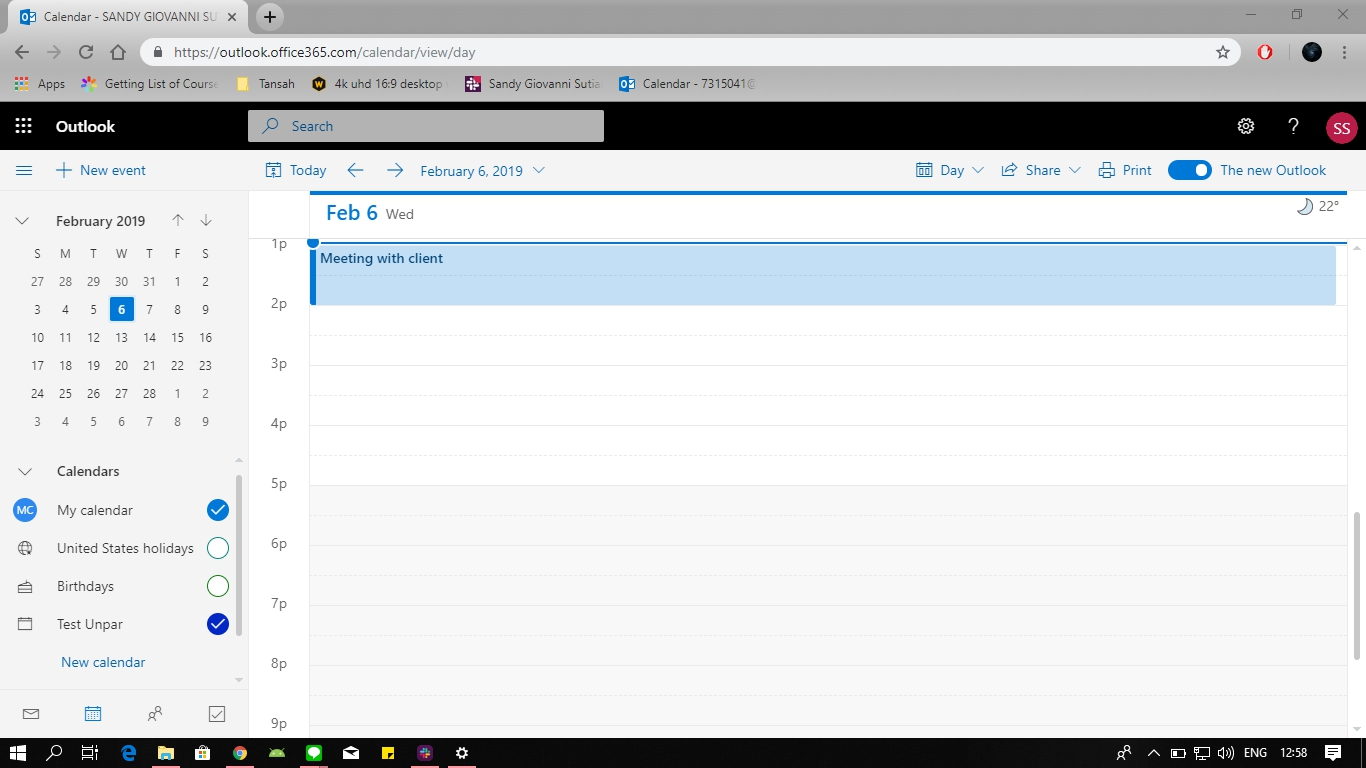
\includegraphics[width=10cm]{img/outlookcalendar.jpg}
  \centering
  \caption{aplikasi \textit{Outlook Calendar}}
\end{figure}

Sedangkan \textit{Slack} sendiri adalah sebuah aplikasi yang berfungsi sebagai \textit{platform} untuk menjalankan \textit{real-time chatting}. 

\begin{figure}[h]
  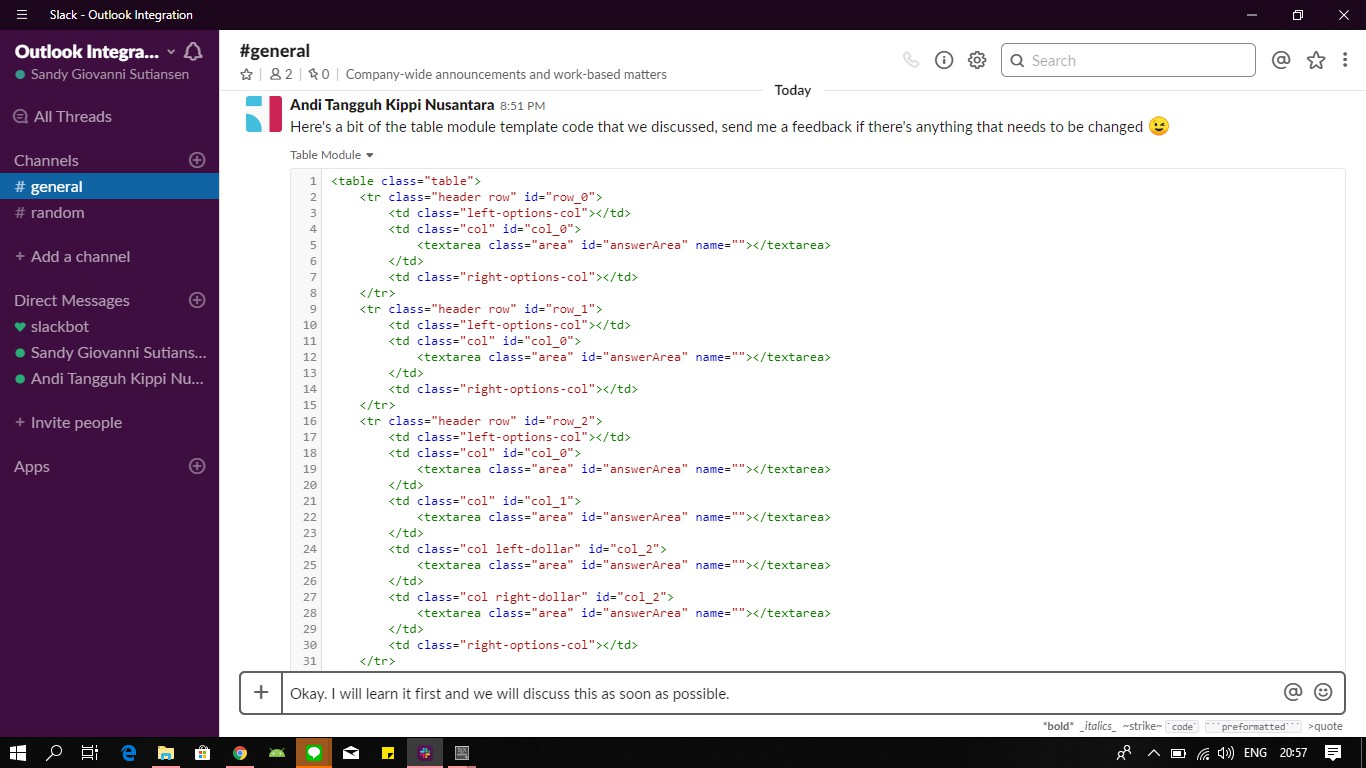
\includegraphics[width=10cm]{img/slack_chat_2.jpg}
  \centering
  \caption{aplikasi \textit{Slack}}
\end{figure}

Yang akan diintegrasikan dari kedua aplikasi itu adalah saat ada \textit{event} yang tercatat di \textit{Outlook Calendar} (seperti di Gambar 1), maka perangkat lunak ini akan membantu untuk mengubah status di dalam aplikasi \textit{Slack}.
\clearpage
\begin{figure}[h!]
\begin{center}
  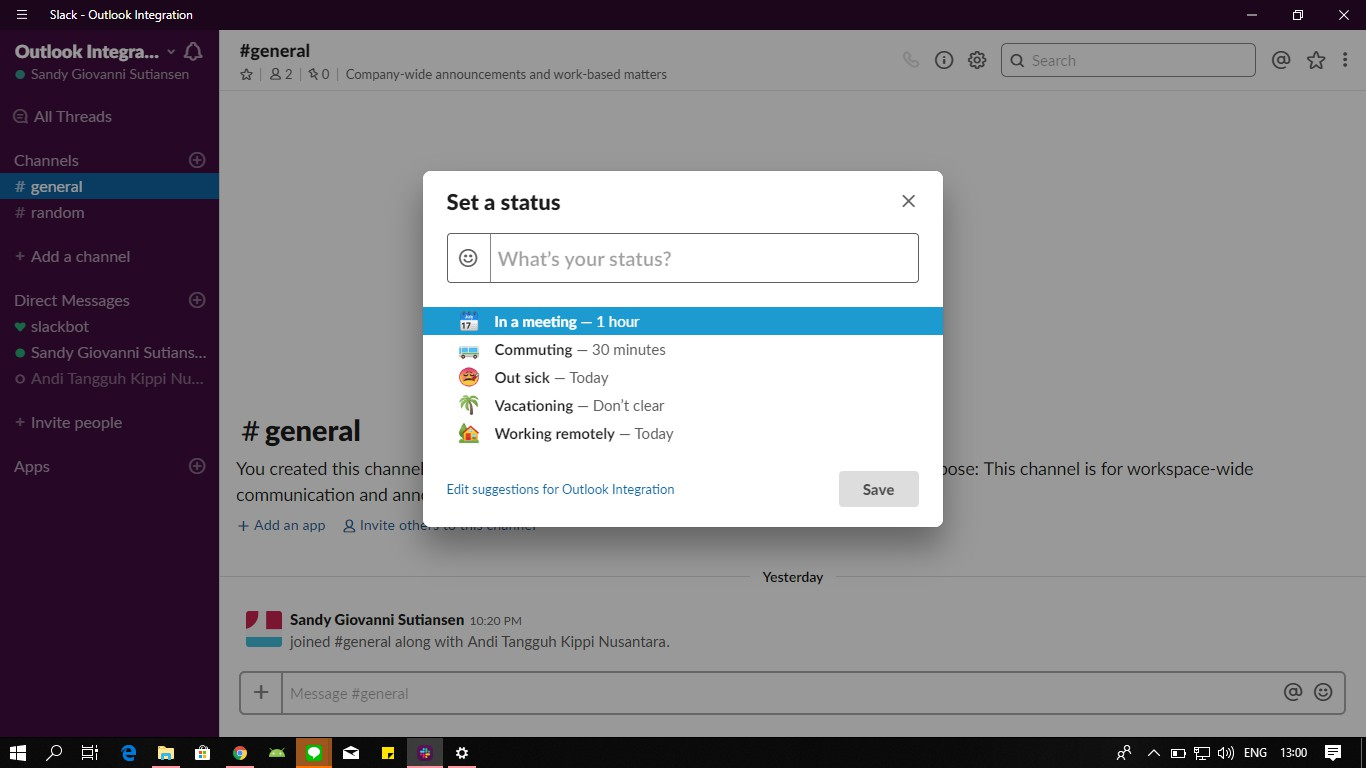
\includegraphics[width=10cm]{img/slack_1.jpg}
  \caption{window pemilihan status di aplikasi \textit{Slack}}
  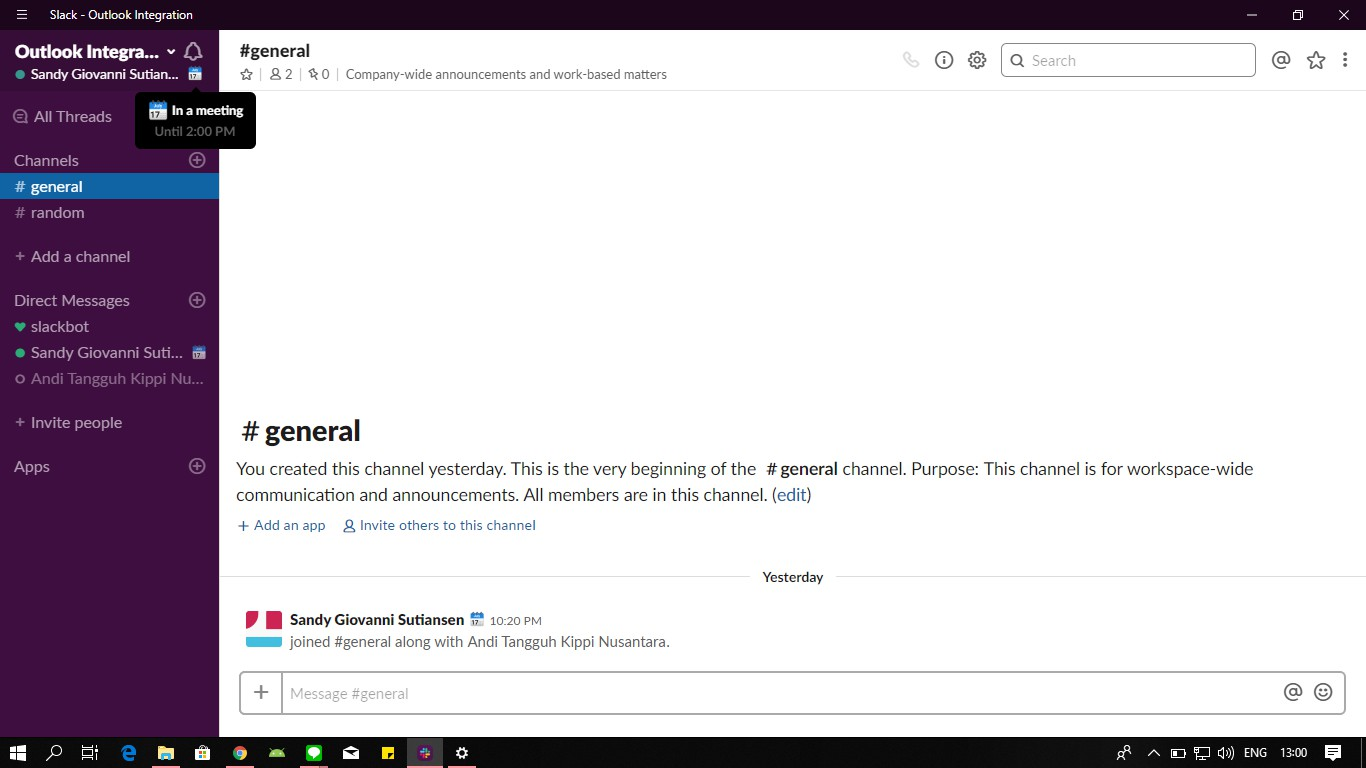
\includegraphics[width=10cm]{img/slack_2.jpg}
  \caption{tampak status dari \textit{icon} yang di \textit{hover}}
  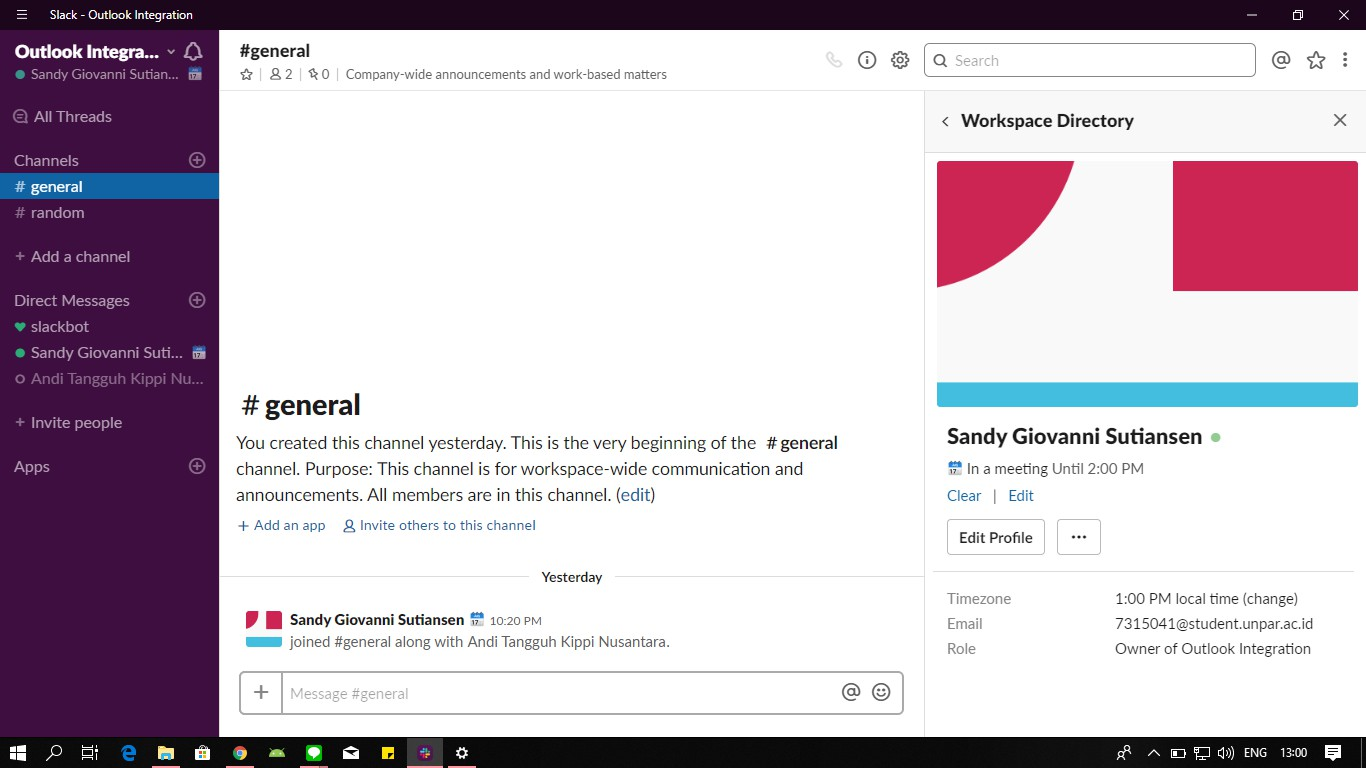
\includegraphics[width=10cm]{img/slack_3.jpg}
  \caption{tampak status dari \textit{profile section}}
\end{center}
\end{figure}

Latar belakang disusunnya aplikasi ini adalah untuk membantu \textit{syncronize} akun \textit{Slack} agar bisa terlihat dalam status tertentu oleh \textit{partner}/ rekan satu tim jika \textit{user} lupa untuk mengubah status yang ada di dalam akun \textit{Slack}-nya saat terdapat jadwal di aplikasi \textit{Outlook Calendar}. 

Perangkat lunak ini akan dibuat dengan bantuan dari masing- masing API (\textit{Application Programming Interface}). \textit{Outlook Calendar} dan juga \textit{Slack} memiliki API masing- masing yang cara penggunaannya terdapat dalam dokumentasi dari aplikasi tersebut yang bisa ditemui di dalam laman \textit{website} dari masing- masing aplikasi tersebut. Perangkat ini juga akan dibangun menggunakan \textit{Node.js} yang bisa dipelajari melalui laman \textit{website} dokumentasi \textit{Node.js} itu sendiri. 

\section{Rumusan Masalah}
Pada perangkat lunak ini, terdapat rumusan masalah sebagai berikut:
\begin{itemize}
	\item Bagaimana cara menggunakan \textit{Node.js}?
	\item Bagaimana cara mendapatkan data \textit{event} dari \textit{Outlook Calendar}?
	\item Bagaimana mengubah status pada aplikasi \textit{Slack} menggunakan \textit{Slack} API?  
	\item Bagaimana cara membuat program agar dapat mengubah status pada aplikasi \textit{Slack} di jadwal yang telah didapat dari aplikasi \textit{Outlook Calendar}? 
	
\end{itemize}

\section{Tujuan}
Adapun pada perangkat lunak ini memiliki tujuan sebagai berikut:
\begin{itemize}
	\item Mengetahui cara menggunakan \textit{Node.js}. 
	\item Mengetahui cara mendapatkan data \textit{event} dari \textit{Outlook Calendar}.   
	\item Mengetahui cara mengubah status pada aplikasi \textit{Slack} menggunakan \textit{Slack} API. 
	\item Mengetahui cara membuat program agar dapat mengubah status pada aplikasi \textit{Slack} di jadwal yang telah didapat dari aplikasi \textit{Outlook Calendar}.  
	
\end{itemize}

\section{Deskripsi Perangkat Lunak}
Pada perangkat lunak ini, nantinya akan memiliki fitur- fitur sebagai berikut:
\begin{itemize}
	\item \textit{Synchronize} \textit{Outlook Calendar} secara berkala. 
	\item Mengubah status sesuai dengan apa yang akan ditentukan oleh \textit{user} saat ada \textit{event} yang sedang berlangsung yang tercatat di \textit{Outlook Calendar}. 
	\item Menghapus status/ mengembalikkan status ke semula saat \textit{event} yang terjadwalkan di \textit{Outlook Calendar} telah berakhir. 
	
\end{itemize}

\section{Detail Pengerjaan Skripsi}
Bagian-bagian pekerjaan skripsi ini adalah sebagai berikut :
	\begin{enumerate}
		\item Melakukan studi literatur melalui dokumentasi \textit{online} mengenai \textit{Node.js}.
		\item Melakukan studi literatur melalui dokumentasi \textit{online} mengenai aplikasi \textit{Outlook Calendar}.
		\item Melakukan studi literatur melalui dokumentasi \textit{online} mengenai aplikasi \textit{Slack}. 
		\item Melakukan analisis cara melakukan \textit{synchronize} dengan aplikasi \textit{Outlook Calendar} secara berkala.
		\item Melakukan analisis cara aplikasi merespons ketika menjadwalkan perubahan status di aplikasi \textit{Slack}, dengan kemungkinan masalah seperti : ada \textit{event} yang baru ditambahkan setelah program melakukan \textit{synchronize} secara berkala atau ada \textit{event} yang beririsan dengan \textit{event} lainnya sehingga terdapat masalah menentukan kapan status dibuang/ dikembalikan lagi ke status semula. 
		\item Merancang bagian dari perangkat lunak yang akan mengambil data- data \textit{event} dari \textit{Outlook Calendar}. 
		\item Merancang bagian dari perangkat lunak yang bertugas untuk mengubah status pada \textit{Slack} saat waktu sesuai dengan jadwal yang sudah tercatat dari \textit{Outlook Calendar}.
		\item Mengimplementasi bagian pengambilan data dari \textit{Outlook Calendar} dan juga bagian mengatur status pada \textit{Slack} sesuai jadwal yang telah diambil kepada perangkat lunak Integrasi \textit{Outlook Calendar} dengan \textit{Slack}.
		\item Melakukan pengujian terhadap fitur yang telah diimplementasi.
		\item Menulis dokumen skripsi.   
	\end{enumerate}

\section{Rencana Kerja}
Rincian capaian yang direncanakan di Skripsi 1 adalah sebagai berikut:

\begin{enumerate}
\item Melakukan studi literatur melalui dokumentasi \textit{online} mengenai \textit{Node.js}.
		\item Melakukan studi literatur melalui dokumentasi \textit{online} mengenai aplikasi \textit{Outlook Calendar}.
		\item Melakukan studi literatur melalui dokumentasi \textit{online} mengenai aplikasi \textit{Slack}. 
		\item Melakukan analisis cara melakukan \textit{synchronize} dengan aplikasi \textit{Outlook Calendar} secara berkala.
		\item Melakukan analisis cara aplikasi merespons ketika menjadwalkan perubahan status di aplikasi \textit{Slack}, dengan kemungkinan masalah seperti : ada \textit{event} yang baru ditambahkan setelah program melakukan \textit{synchronize} secara berkala atau ada \textit{event} yang beririsan dengan \textit{event} lainnya sehingga terdapat masalah menentukan kapan status dibuang/ dikembalikan lagi ke status semula. 
\end{enumerate}

Sedangkan yang akan diselesaikan di Skripsi 2 adalah sebagai berikut:

\begin{enumerate}
\item Merancang bagian dari perangkat lunak yang akan mengambil data- data \textit{event} dari \textit{Outlook Calendar}. 
		\item Merancang bagian dari perangkat lunak yang bertugas untuk mengubah status pada \textit{Slack} saat waktu sesuai dengan jadwal yang sudah tercatat dari \textit{Outlook Calendar}.
		\item Mengimplementasi bagian pengambilan data dari \textit{Outlook Calendar} dan juga bagian mengatur status pada \textit{Slack} sesuai jadwal yang telah diambil kepada perangkat lunak Integrasi \textit{Outlook Calendar} dengan \textit{Slack}.
		\item Melakukan pengujian terhadap fitur yang telah diimplementasi.
		\item Menulis dokumen skripsi.
\end{enumerate}
\clearpage

\vspace{1cm}
\centering Bandung, \tanggal\\
\vspace{2cm} \nama \\ 
\vspace{1cm}

Menyetujui, \\
\ifdefstring{\jumpemb}{2}{
\vspace{1.5cm}
\begin{centering} Menyetujui,\\ \end{centering} \vspace{0.75cm}
\begin{minipage}[b]{0.45\linewidth}
% \centering Bandung, \makebox[0.5cm]{\hrulefill}/\makebox[0.5cm]{\hrulefill}/2013 \\
\vspace{2cm} Nama: \makebox[3cm]{\hrulefill}\\ Pembimbing Utama
\end{minipage} \hspace{0.5cm}
\begin{minipage}[b]{0.45\linewidth}
% \centering Bandung, \makebox[0.5cm]{\hrulefill}/\makebox[0.5cm]{\hrulefill}/2013\\
\vspace{2cm} Nama: \makebox[3cm]{\hrulefill}\\ Pembimbing Pendamping
\end{minipage}
\vspace{0.5cm}
}{
% \centering Bandung, \makebox[0.5cm]{\hrulefill}/\makebox[0.5cm]{\hrulefill}/2013\\
\vspace{2cm} Nama: \makebox[3cm]{\hrulefill}\\ Pembimbing Tunggal
}
\end{document}

